%%%%%%%%%%%%%%%%%%%%%%%%%%%%%%%%%%%%%%
%% Header section of Latex document %%
%%%%%%%%%%%%%%%%%%%%%%%%%%%%%%%%%%%%%%

\documentclass[runningheads,a4paper,11pt]{report}

\usepackage{pgf-umlsd}
\usepackage{listings}
\usepackage{tikz}
\usepackage{pgfplots}
\usepackage{pgfplotstable}
\usepackage[numbers]{natbib}
\usepackage{graphicx}
\usepackage{subcaption}

\usepgfplotslibrary{statistics}


\usepackage[a4paper]{geometry}
\usepackage{t1enc}
\usepackage[utf8]{inputenc}
\usepackage{lmodern}

\usepackage[title,titletoc]{appendix}
\usepackage[section]{placeins}
\usepackage{relsize}

\usepackage[normalem]{ulem} %% Provides underlining.
\usepackage{caption} %% Provides captions.
\usepackage{mdframed} %% Provides frames around text and equations.
\usepackage{tikz-cd} %% Provides diagram drawing environment.
\usepackage{adjustbox} %% Provides additional tools to resize content.
% \usepackage[magyar]{babel} %% Provides foreign language support.

%%%%
%% Provides math related environments and directives.
\usepackage{amssymb}
\usepackage{amsthm}
\usepackage{amsmath}
\usepackage{latexsym}

\usepackage{dsfont}
\usepackage{commath}
\usepackage{bm}
\usepackage{subcaption}
\usepackage{upgreek}

%% See http://tex.stackexchange.com/questions/43835/conflict-between-amsthm-and-some-other-package
\let\proof\relax 
\let\endproof\relax

%%%%
%% Provides table environments and related directives.
\usepackage{array}
\usepackage{tabulary}
\usepackage{tabularx}
\usepackage{multirow}
\usepackage{hhline}
\usepackage{diagbox}
\usepackage{array}

%%%%
%% Provides figure environments and related directives.
\usepackage{graphicx}
\makeatletter
\def\maxwidth#1{\ifdim\Gin@nat@width>#1 #1\else\Gin@nat@width\fi}
\def\maxheight#1{\ifdim\Gin@nat@height>#1 #1\else\Gin@nat@height\fi}
\makeatother

\usepackage{fancyvrb}
\usepackage{rotating}

%%%%
%% Provides environment to display source code.
\usepackage{listings} 
\lstset{ 
    literate=%
        {á}{{\'a}}1
        {é}{{\'e}}1
        {í}{{\'i}}1
        {ó}{{\'o}}1
        {ö}{{\"o}}1
        {ő}{{\H{o}}}1
        {ú}{{\'u}}1
        {ü}{{\"u}}1
        {ű}{{\H{u}}}1
        {Á}{{\'A}}1
        {É}{{\'E}}1
        {Í}{{\'I}}1
        {Ó}{{\'O}}1
        {Ö}{{\"O}}1
        {Ő}{{\H{O}}}1
        {Ú}{{\'U}}1
        {Ü}{{\"U}}1
        {Ű}{{\H{U}}}1
    } %% Customization of listings env., to enable non-English accents.

\lstset{
   frame=single,
   basicstyle=\small,
   language=Erlang,
   numbers=left,
   firstnumber=1,
   numberfirstline=true,
%  basicstyle=\ttfamily,
%  columns=fullflexible,
%   keepspaces=true,
} %% Customization of listings environment


%%%%
%% Provides environment to display pseudocode.
\usepackage{algorithm}% http://ctan.org/pkg/algorithms
\usepackage{algpseudocode}% http://ctan.org/pkg/algorithmicx

\newcommand{\repeatcaption}[2]{%
  \addtocounter{figure}{-1}%
  \renewcommand{\thefigure}{\ref{#1}}%
  \captionsetup{list=no, labelformat=simple, labelsep=colon}%
  \captionof{figure}{#2}%
} %% Customization: Using the same figure twice with no new number. See http://tex.stackexchange.com/a/200229

\newcommand{\N}{\mathbb{N}}
\newcommand{\Z}{\mathbb{Z}}
\newcommand{\R}{\mathbb{R}}
\newcommand{\C}{\mathbb{C}}
\newcommand{\Hq}{\mathbb{H}}
\newcommand{\D}{\mathbb{D}}

\newcommand{\qi}{\textbf{i}}
\newcommand{\qj}{\textbf{j}}
\newcommand{\qk}{\textbf{k}}
\newcommand{\qmu}{\boldsymbol{\mu}}

\DeclareMathOperator{\rp}{Re}
\DeclareMathOperator{\ip}{Im}

%%%%
%% Provides directives to display followable URL references.
\usepackage{url}
\usepackage{hyperref}
\hypersetup{
  hidelinks,
  linkbordercolor = {0 0 1},
}

%% Customization: Followable links to appendix references.
\makeatletter
\appto{\appendices}{\def\Hy@chapapp{Appendix}}
\makeatother


%%%%
%% Custom document formatting.

% \renewcommand{\abstract}{ \begin{center}\textbf{Abstract}\end{center}}

\setcounter{tocdepth}{2}

\setlength{\parskip}{\baselineskip}%
\setlength{\parindent}{0pt}%

\makeatletter
\renewcommand\subsection{\@startsection{subsubsection}{3}{\z@}%
                       {-18\p@ \@plus -4\p@ \@minus -4\p@}%
                       {4\p@ \@plus 2\p@ \@minus 2\p@}%
                       {\normalfont\normalsize\bfseries\boldmath
                        \rightskip=\z@ \@plus 8em\pretolerance=10000 }}
\makeatother


%%%%
%% Custom theorem environments.
\newtheorem{mydef}{Definition}
\newtheorem{myexamp}{Example}

%%%%
%% Custom symbol definitions and abbreviations.
\makeatletter
\providecommand{\leadsfrom}{%
  \mathrel{\mathpalette\reflect@squig\relax}%
}
\newcommand{\reflect@squig}[2]{%
  \reflectbox{$\m@th#1\leadsto$}%
}
\makeatother

\renewcommand{\labelitemi}{$\circ$}
\newcommand{\edge}[1]{\stackrel{\bf{#1}}{\rightarrow}}
\newcommand{\ledge}[1]{\stackrel{\bf{#1}}{\leftarrow}}
\newcommand{\rel}[1]{\stackrel{\bf{#1}}{\leadsto}}
\newcommand{\trel}[1]{\stackrel{\bf{#1}}{\leadsto^*}}
\newcommand{\lrel}[1]{\stackrel{\bf{#1}}{\leadsfrom}}

\newcommand{\eqname}[1]{\tag*{#1}}% Tag equation with name

\newcommand{\nv}[0]{node(v)}
\newcommand{\ruleref}[1]{(\S\ref{#1})}
\newcommand{\apxref}[1]{(Appendix \ref{#1}.)}
\newcommand{\apxrefm}[3]{(Appendix \ref{#1}., \ref{#2}. és \ref{#3}.)}


\usepackage[utf8]{inputenc}
\usepackage{enumitem}
\usepackage{hyperref}
\usepackage{bashful}
\usepackage{setspace}
\usepackage{color}
\usepackage{xcolor}

\definecolor{codegreen}{rgb}{0,0.6,0}
\definecolor{codegray}{rgb}{0.2,0.2,0.2}
\definecolor{codeblue}{rgb}{0.0,0,0.62}
\definecolor{backcolour}{rgb}{0.95,0.95,0.95}

\newcommand{\lstbasicfont}{\small\fontfamily{pcr}\selectfont}
\newcommand{\lstcommentstyle}{\color{codegreen}\itshape}

\lstdefinestyle{mystyle}{
    backgroundcolor=\color{backcolour},
    commentstyle=\lstcommentstyle,
    keywordstyle=\color{codeblue}\bfseries,
    %identifierstyle=\color{black},
    identifierstyle=\color{codegray}\bfseries,
    %numberstyle=\tiny\color{codegray},
    stringstyle=\color{purple},
    basicstyle=\lstbasicfont,
    %basicstyle=\small\ttfamily,
    breakatwhitespace=false,
    breaklines=true,
    captionpos=b,
    keepspaces=true,
    %numbers=left,
    %numbersep=5pt,
    showspaces=false,
    showstringspaces=false,
    showtabs=false,
    tabsize=2
}

%% To remove syntax highlighting of Erlang codes
%% uncomment the two commented lines
\lstdefinelanguage{myerlang}[]{erlang}{
  morekeywords={spec,fun,bitstring,orelse,andalso,record,include_lib,begin,end},
  otherkeywords={|,||,<-,->,!,[,],\{,\}},
  deletekeywords={list,ok},
%   identifierstyle=\ttfamily,
%   keywordstyle=\ttfamily
}

\lstset{style=mystyle,
literate=
  {∪}{{$\cup$}}1 {∩}{{$\cap$}}1 {∈}{{$\in$}}1 {⊆}{{$\subseteq$}}1
  {∘}{{$\circ$}}1 {-}{{-}}1 {~}{{\texttildelow}}1 {<}{{<}}1
  {>}{{>}}1
}

%%%%%%%%%%%%%%%%%%%%%%%%%%%%%%%%%%%%
%% Body section of Latex document %%
%%%%%%%%%%%%%%%%%%%%%%%%%%%%%%%%%%%%
\pgfplotsset{compat=1.13}
\begin{document}

% \thispagestyle{empty}
% \begin{center}
% {\Huge TDK dolgozat}\\[0.5cm]
% {\bf Nagy Gergely} \\[1cm]
% \end{center}


\begin{titlepage}
  \noindent
  \begin{minipage}{0.25 \textwidth}
    
\includegraphics[height=40mm]{figures/cimer.png}
  \end{minipage}
  \hfill
  \begin{minipage}{0.67 \textwidth}
    \large
    Eötvös Loránd University \\
    Faculty of Informatics \\
    Department of Numerical Analysis \\
    
  \end{minipage}

  \vfill

  \begin{center}
    {\LARGE \bfseries Color image analysis and recognition using Zernike moments} 
    % \\[0.5cm]
    \\[2.0cm]
    {\Large TDK thesis}
    \\[3cm]
    %%\\[6cm]
    \begin{minipage}[t]{0.45 \textwidth}
      \emph{Supervisor:} \\[0.25 \baselineskip]
      {\large Zsolt Németh} \\[0.5 \baselineskip]
      Title title title
    \end{minipage}
    \begin{minipage}[t]{0.45 \textwidth}
      \begin{flushright}
        \emph{Author:} \\[0.25 \baselineskip]
        {\large Gergely Nagy} \\[0.5 \baselineskip]
        Computer Science MSc \\ %% The name of your program
        1\textsuperscript{st} year
      \end{flushright}
    \end{minipage}
  \end{center}

  \vfill

  \begin{center}
    \large Budapest

    % \large Date of closing: 23 May 2019 
  \end{center}
\end{titlepage}

%%%%%%%%%%%%%%%%%%%%%%%%%%%%%%%%%
%% Content sections start here %%

\begin{abstract}
Image moments and moment invariants are widely used in applications for pattern matching, image recognition, or feature extraction.

Most of the classical moments are defined for grayscale images, however, extending these techniques to multichannel ones is a generally unresolved problem. Conventionally, for color images either RGB decomposition or grayscale conversion was used.

More recently, the algebra of quaternions has been used to extend the grayscale methods to color images. Quaternion Zernike moments have been introduced as an extension of Zernike moments~\cite{qzm}. These Zernike moments are defined by the Zernike functions, which are a system of orthogonal functions over the unit disk, possessing certain inherent invariance properties.

The method for discretizing quaternion Zernike moments in works \cite{qzm} and \cite{qzmi} introduces uniformly distributed points over the unit disk. This method does not achieve discrete orthogonality, which is an important property of the discretization of methods defined by orthogonal functions.

In this thesis, we propose a novel method for the discretization of quaternion Zernike moments over the unit disk: a system of points is defined on the unit disk, over which the quaternion Zernike functions are discrete orthogonal. This improves the robustness of computing the moments by decreasing the error introduced by discretization.

The new method is compared to the original one. In the case of image reconstruction, we find that the novel method decreases the error of reconstruction significantly.

The recognition capabilities for rotated, scaled and translated images with varying levels of noise are also studied. We find that with respect to Gaussian noise the new method achieves significantly better rates of recognition, even for high noise values.
\end{abstract}

\tableofcontents

\chapter{Introduction}
\label{sec:intro}
Moment invariants are widely used in applications for pattern matching~\cite{app2}, image recognition~\cite{pattern_recognition}, or to extract useful features from images~\cite{zernike_nn}.

Most of the moments are defined for single-channel, grayscale images, however extending these techniques to multichannel color images is an important and generally unresolved problem with many possible applications. Conventionally, for color images either RGB decomposition or grayscale conversion was used in order to utilize the methods defined for grayscale images. This may lead to loss of information, for example in the case of grayscale conversion (where the average of the color channels is taken) some color information can be lost.

More recently, the algebra of quaternions has been used to extend the single-channel methods to color images. For example, quaternion Fourier-Mellin moments have been introduced as an extension of the conventional Fourier-Mellin moments~\cite{qfmm}, as well as the quaternion Zernike moments as an extension of the conventional Zernike moments~\cite{qzm}.

The Zernike functions are a system of orthogonal functions defined over the unit disk. Using these functions as a basis for series expansions proved to be useful because of certain inherent invariance properties. Zernike moments, and by extension quaternion Zernike moments are defined by these functions.

Considering a digital image as a discrete sampling of an image function defined over a continuous domain, the need arises to discretize the computation of these moments. One important property of the discretization of these methods defined by orthogonal functions is to preserve the orthogonality over the discrete system, so as to avoid redundancy and achieve high robustness with respect to noise.

The conventional method for discretizing quaternion Zernike moments (used by \citeauthor{qzmi}~\cite{qzmi}) consists of uniformly distributed points over the unit disk. This method does not achieve discrete orthogonality thus decreasing the robustness of the moments. 

Our goal was to create a system over which the quaternion extension of the Zernike functions is discrete orthogonal and thus improve the robustness of quaternion Zernike moments and to decrease the error introduced by discretization.


\section{Contributions}
In this thesis a new method is proposed for the discretization of quaternion Zernike moments over the unit disk. A point system is constructed on the unit disk, over which the Zernike functions extended to quaternions are discrete orthogonal. 

This new method is compared to the method used by \citeauthor{qzmi}~\cite{qzmi}. For the tests, image sets from the Columbia Object Image Library~\cite{coil} and the Amsterdam Library of Object Images~\cite{aloi} were used. 

Besides the theoretical invariance properties of QZMIs, these are also verified empirically. The image reconstruction capabilities of both methods are compared and we find that the proposed method decreases the error of reconstruction significantly.

The methods are also applied to the recognition of rotated, scaled and translated (RST transformed) images with varying levels of either Gaussian or salt-and-pepper noise. We find that with respect to Gaussian noise the new method achieves significantly better rates of recognition, even for images with high noise values. For salt-and-pepper noise no significant difference can be found between the capabilities of the methods.
Additionally, we also show that by decreasing the number of points used for discretization, the new method is able to achieve similar results as the original method with high number of points, but the computational need to obtain these results is much lower using the new method.


\section{Structure of the thesis}
This section serves as an overview of the structure of this thesis and contains a short summary of each chapter.

Chapter~\ref{sec:intro} serves as an introduction, where the motivation for this work is described and the contributions featured in this thesis are presented.

Chapter~\ref{sec:background} provides the background for our work. The core concepts, such as (quaternion) Zernike moments and invariants are described in detail. A summary of previous methods for the discretization of quaternion Zernike moments is also given. Finally, some applications relying on Zernike moments are described.

The method we propose for the discretization of Zernike moments is presented in Chapter~\ref{sec:maths}. The construction of a discrete orthogonal point system and the proof of discrete orthogonality is also given.

The different methods and technologies used for the computation of the invariants is shown in Chapter~\ref{sec:implementation}. The computation of the proposed new system is also described.

Chapter~\ref{sec:tests} contains the description of all the tests conducted on the methods, such as image reconstruction or recognition. The results of these tests are evaluated and the original and proposed methods are compared.

Finally, Chapter~\ref{sec:conclusion} summarizes the work and results presented in this thesis. Future development possibilities are also presented.

\chapter{Background}
\label{sec:background}
TODO Background

Image moments in general

Explain Zernike moments

QZMI, QZMRI:
greyscale, color, etc

examples, use cases


\chapter{Math?}
In this chapter we describe our proposed approach to the discretization of continuous quaternion Zernike moments. Our aim is to ensure simple and reversible computability, but achieve considerable reduction in potential computational inaccuracies at the same time. For this, we define a system of sampling points $(r_k,\theta_j)$, over which the integral discretization \eqref{eq:QZMappr} maintains advantageous theoretical properties. The idea behind our approach is motivated by the work \cite{schipp}.

Fix a positive integer $N$. Let us denote by $\rho_{k,N}$, $k=1,\ldots,N$ the roots of the N-th order Legendre polynomial \cite{Szego}. Notating the fundamental polynomials of Lagrange interpolation with respect to the roots $\rho_{k,N}$ as $\ell_{k,N}$, we define the constants
\[
	\mathcal{A}_{k,N} = \int_{-1}^{1} \ell_{k,N}(x)\ dx, \qquad (k=1,\ldots,N).
\]

Then, the system of sampling points $X_N$ over the unit disk $\D$ is defined in polar form by
\[
	X_N\ni (r_{k,N}, \theta_{j,N}) = \left(\sqrt{\frac{1+\rho_{k,N}}{2}} , \frac{2\pi j}{4N} \right), \qquad (k=1,\ldots,N,j=1,\ldots,4N),
\]
and the respective weight values and constants are
\[
	w(r_{k,N},\theta_{j,N}) = \frac{\mathcal{A}_{k,N}}{8N},\qquad \lambda_{n,m} = n+1,
\]
so the generated integral approximation based on \eqref{eq:QZMappr} is
\[
	\frac{1}{\pi} \int_{0}^1 \int_0^{2\pi} f(r,\theta)\ d\theta dr \approx \int_{X_N} f = \sum_{k=1}^{N} \sum_{j=1}^{4N} f(r_{k,N},\theta_{j,N}) \frac{\mathcal{A}_{k,N}}{8N}.
\]
We remark that the values $\mathcal{A}_{k,N}$ are somewhat close to $\frac{1}{N}$, so the weighting is close to being uniform.

What is appealing in this choice of $X_N$ is the fact that the orthogonality of quaternion Zernike functions \eqref{QZortho} is preserved under changing to  discrete integration over this set of points, i.e.
\begin{theorem}\label{QZdisc-ortho}
Suppose that for $n,n' \in \N$ naturals and $m,m' \in \Z$ integers we have $$\frac{n+n'}{2}+\min(|m|,|m'|) < 2N.$$ Then
\[
	(n+1) \int_{X_N} \phi_{n,m} \phi^*_{n',m'} =\delta_{n,n'}\delta_{m,m'}.
\]
\end{theorem}
\noindent\textbf{Proof.}
Let us consider the radial orthogonality relation \eqref{Rortho} expressed with the Jacobi polynomials of \eqref{RJacobi}, i.e.
\[
\begin{gathered}
	\frac{1}{2n+2} \delta_{n,n'} = \int_0^1 R_{n,|m|}(r) R_{n',|m|}(r)r\ dr  = \\
	\int_0^1 r^{2|m|} P_{\frac{n - |m|}{2}}^{(0,|m|)}(2r^2-1) P_{\frac{n' - |m|}{2}}^{(0,|m|)}(2r^2-1) r\ dr,
\end{gathered}
\]
and apply a change of variable $u=2r^2-1$, to obtain
\[
	\frac{1}{2n+2} \delta_{n,n'} = \frac{1}{4} \int_{-1}^1 \left(\frac{1+u}{2}\right)^{2|m|} P_{\frac{n - |m|}{2}}^{(0,|m|)}(u) P_{\frac{n' - |m|}{2}}^{(0,|m|)}(u)\ du.
\]
Notice that here the integrand is a polynomial of degree $\frac{n+n'}{2}+|m| < 2N$, so the exact value of the integral is equal to the value of the Gauss-Legendre quadrature (see e.g. \cite{Szego}), i.e.
\[
	\frac{1}{2n+2} \delta_{n,n'} = \frac{1}{4} \sum_{k=1}^{N} \mathcal{A}_{k,N} \left(\frac{1+\rho_{k,N}}{2}\right)^{2|m|} P_{\frac{n - |m|}{2}}^{(0,|m|)}(\rho_{k,N}) P_{\frac{n' - |m|}{2}}^{(0,|m|)}(\rho_{k,N}).
\]

Rewriting this in terms of $r_{k,N} = \sqrt{\frac{1+\rho_{k,N}}{2}}$ gives a discrete orthogonality relation for the radial polynomials, as
\begin{equation}\label{Rdisc-ortho}
	\frac{1}{2n+2} \delta_{n,n'} = \frac{1}{4} \sum_{k=1}^{N} \mathcal{A}_{k,N} R_{n,m}(r_{k,N}) R_{n',m}(r_{k,N}).
\end{equation}

Now we can proceed with proving the statement. 
\[
\begin{gathered}
	\int_{X_N} \phi_{n,m} \phi^*_{n',m'} = \sum_{k=1}^{N} \sum_{j=1}^{4N} \phi_{n,m}(r_{k,N},\theta_{j,N}) \phi^*_{n',m'}(r_{k,N},					\theta_{j,N}) \frac{\mathcal{A}_{k,N}}{8N} = \\
	\frac{1}{8N} \left( \sum_{j=1}^{4N} e^{-\qmu m\theta_{j,N}}e^{\qmu m' \theta_{j,N}} \right) \left( \sum_{k=1}^N \mathcal{A}_{k,N} R_{n,m}(r_{k,N}) R_{n',m'}(r_{k,N}) \right),
\end{gathered}
\]
and since quaternions $-\qmu m\theta_{j,N}$ and $\qmu m' \theta_{j,N}$ commute, we have
\[
	\sum_{j=1}^{4N} e^{-\qmu (m-m')\frac{2\pi j}{4N}} = 4N\delta_{m,m'}
\]
for the first sum, so if $m\neq m'$, the discrete integral equals to $0$ and we are done.

Suppose $m=m'$, now we are left with
\[
	\int_{X_N} \phi_{n,m} \phi^*_{n',m} = \frac{1}{2} \sum_{k=1}^N \mathcal{A}_{k,N} R_{n,m}(r_{k,N}) R_{n',m}(r_{k,N}) = \frac{1}{n+1}\delta_{n,n'},
\]
where we used \eqref{Rdisc-ortho} for the last equation as we have $\frac{n+n'}{2}+|m| < 2N$.
\qed

Theoretically, the discrete orthogonality relation of Theorem \ref{QZdisc-ortho} means that the exact values of right and left moments can be computed, provided we can measure the function values over $X_N$, for a sufficiently large $N$: let us consider an arbitrary linear combination of right moments \eqref{eq:QZRM} in the form
\[
	f \approx f_N(r,\theta) = \mathop{\sum\sum}_{n+m<2N} Z^R_{n,m}(f) \phi^*_{n,m} (r,\theta),
\]
then the exact value of the moment $Z^R_{n,m}(f)$, using the previous result, is
\[
	Z^R_{n,m}(f) = \int_{X_N} f_N\phi_{n,m},
\]
and the same can be said for the left moments. This proves that for system $X_N$, the discretization error is zero, a property that no other previously used quaternion moment method possessed. Besides this, only numerical roundoffs and the moment order threshold $f \approx f_N$ generates computational inaccuracies.

\chapter{Implementation}
This chapter presents the tools and methods used for implementing a program for calculating the QZMIs of an image using both methods of discretization.

\section{Programming language and libraries used}
The implementation was created using the Python programming language~\cite{python} and relying on the Numpy~\cite{numpy} and Numba~\cite{numba} libraries to achieve efficient and fast computation of the moment invariants, as well as the Python Imaging Library (PIL, Pillow)~\cite{pil} for image manipulation.

Numpy provided a way to efficiently work with arrays and matrices. It also provided the quaternion package, which supports the quaternion data type.

Using the just-in-time compilation (JIT) capabilities of Numba (i.e. the \texttt{@jit} annotation), the computationally heavy parts of the implementation could be made almost as fast as native code. The disadvantage of using JIT is that it limits the available types and functions, so in the implementation the use of \texttt{@jit} is kept only to the critical, computationally intensive functions. 

\section{Calculating moments and moment invariants}
\begin{figure}[tbp]
    \centering
        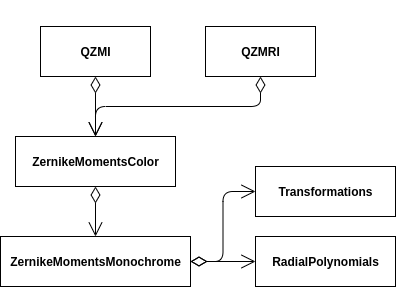
\includegraphics[width=0.5\textwidth]{figures/qzmi_classes.png}
    \caption{The relationships between the classes used to calculate QZMIs and QZMRIs}
    \label{fig:classes}
\end{figure}
To obtain the quaternion Zernike moment invariants (QZMIs) of an image as described in Section~\ref{sec:invariance}, the quaternion Zernike moments (QZMs) must be calculated first. \citeauthor{qzmi}~\cite{qzmi} showed that instead of calculating the QZMs directly by using the algebra of quaternions, it is possible to calculate the real and the imaginary parts of the quaternion-valued QZM individually by using some linear combination of the real and imaginary parts of the complex-valued, single channel Zernike moments. This means that the single channel Zernike moments have to be calculated for all three of the RGB color channels.
Furthermore, the calculation of the Zernike moments requires the computation of the radial polynomials, introduced in~\eqref{eq:radial_poly}.

To calculate the required values, the following four classes were created, each relying on the next one to perform the computation.
\begin{itemize}
    \item \texttt{QZMI}, for calculating the quaternion Zernike moment invariants
    \item \texttt{ZernikeMomentsColor}, for calculating the quaternion-valued Zernike moments
    \item \texttt{ZernikeMomentsMonochrome}, for calculating the complex-valued, single channel Zernike moments
    \item \texttt{RadialPolynomials}, for calculating the values of the radial polynomials at a given point
\end{itemize}
The relationships between these classes are shown on Figure~\ref{fig:classes}, as well as the \texttt{QZMRI} class, which calculates the rotation invariant QZMs needed for some test cases. A description of the algorithms used in these classes and the data stored by them is given below.

Since the work presented in this thesis involves changing the way an image is transformed from image coordinates to polar coordinates inside the unit circle, the classes were made modular with respect to the transformation used. This makes it easy to create and test a new image transformation function with the interface expected by the calculating classes.

\subsection{Radial polynomials}
To calculate the value of all $R_{n,m}$ radial polynomials up to some maximal degree $P$ at a point $r \in [0,1]$, the modified Kintner's method was used, as described in~\cite{kintner}. This algorithm computes the value of $R_{n,m}(r)$ for all $0 \leq |m| \leq n \leq P$, ($n - |m|$ is even) with complexity $\mathcal{O}(N^2)$. This method is ideal for the computation of all radial polynomial values up to a maximum degree.

Since this method is called many times during the calculation of Zernike moments, just-in-time compilation was used to further increase efficiency. Figure~\ref{fig:radial_code} shows the JIT-enabled function.

\begin{figure}[tbp]
    \centering
    \begin{lstlisting}[language=Python]
@jit(void(float64, int32, float64[:,:]), nopython=True)
def calculateRadialPolynomials(r, P, values):
  values[0,0] = 1
  values[1,1] = r
  for n in range(2,P + 1):
    h = n*(n - 1)*(n - 2)
    K2 = 2*h
    values[n,n] = (r**n)
    values[n,n-2] = n*values[n,n] - (n-1)*values[n-2,n-2]
    for m in range(n-4,-1,-2):			
      K1 = (n + m)*(n - m)*(n - 2)/2
      K3 = (-1)*m*m*(n - 1) - h
      K4 = (-1)*n*(n + m - 2)*(n - m - 2)/2
      r2 = r**2
      values[n,m] = ((K2*r2+K3)*values[n-2,m]+K4*values[n-4,m])/K1\end{lstlisting}
    \caption{Function for calculating radial polynomial values}
    \label{fig:radial_code}
\end{figure}

\subsection{Complex Zernike moments}
The \texttt{ZernikeMomentsMonochrome} class calculates the conventional Zernike moments of degree at most $P$ of a square $N \times N$, single channel (grayscale) image. The algorithm is based directly on the discretized definition of the Zernike moments.
For the original linear transformation of the image onto the unit disk, this gives:
\begin{gather*}
    \begin{split}
    Z_{n,m}(f) &= \lambda\frac{(n+1)}{(N-1)^2}\sum_{x=1}^{N}\sum_{y=1}^{N}f(x,y)V_{n,m}^{*}(r_{x,y},\theta_{x,y}) \\
    &= \lambda\frac{(n+1)}{(N-1)^2}\sum_{x=1}^{N}\sum_{y=1}^{N}f(x,y)R_{n,m}(r_{x,y})e^{-\bm{i}m\theta_{x,y}} \\
    &= \lambda\frac{(n+1)}{(N-1)^2}\sum_{x=1}^{N}\sum_{y=1}^{N}f(x,y)R_{n,m}(r_{x,y})(\cos (m\theta_{x,y}) - \bm{i}\sin (m\theta_{x,y}))
    \end{split}
\end{gather*}
where $0\leq |m| \leq n \leq P$, $n - |m|$ is even, $(r_{x,y},\theta_{x,y})$ are the $(x,y)$ coordinates transformed to the unit disk, $\lambda$ is the scaling parameter also given by the transformation (as described in Section~\ref{sec:discretization}) and $f$ is the real-valued, grayscale image.

By precomputing the sin and cos values for all possible $m$ and $\theta_{x,y}$ values, as well as the values of the radial polynomials, this formula gives an efficient way of calculating the real and imaginary parts of the Zernike moments separately. This way only primitive data types have to be used during the computation and it can be made more efficient using JIT.

Also, there is no need to calculate the Zernike moments for negative $m$ values, as the $Z_{n,m}(f) = Z_{n,-m}(f)^{*}$ identity can be used later to obtain those values.

\subsection{Quaternion Zernike moments}
The class \texttt{ZernikeMomentsColor} calculates the quaternion Zernike moments of an RGB image. First, the conventional Zernike moments for each of the three color channels are calculated, then the relationship between QZMs and Zernike moments is used to construct the quaternions~\cite{qzmi}.
\begin{gather*}
    \begin{split}
        Z_{n,m}^R(f) = &-\frac{1}{\sqrt{3}}\left( Im(Z_{n,m}(f_R)) + Im(Z_{n,m}(f_G)) + Im(Z_{n,m}(f_B)) \right)\\
        &+\left[Re(Z_{n,m}(f_R)) + \frac{1}{\sqrt{3}}\left(Im(Z_{n,m}(f_G)) - Im(Z_{n,m}(f_B))\right)\right]\bm{i}\\
        &+\left[Re(Z_{n,m}(f_G)) + \frac{1}{\sqrt{3}}\left(Im(Z_{n,m}(f_B)) - Im(Z_{n,m}(f_R))\right)\right]\bm{j}\\
        &+\left[Re(Z_{n,m}(f_B)) + \frac{1}{\sqrt{3}}\left(Im(Z_{n,m}(f_R)) - Im(Z_{n,m}(f_G))\right)\right]\bm{k}\\
    \end{split}
\end{gather*}
where $f$ is an RGB image and $f_R, f_G, f_B$ are the red, green and blue color channels respectively.

Again, only the QZMs $Z_{n,m}^R$ ($m \geq 0$) are calculated, because for $m < 0$ the $Z_{n,m}^R(f) = Z_{n,-m}^R(f)^{*}$ equality can be used.

\subsection{Invariants}
The class \texttt{QZMI} is responsible for computing the combined rotation, scaling and translation (RST) invariant moments, while the class \texttt{QZMRI} computes the moments which are invariant only to rotation.
The invariants for scaling and rotation are calculated directly using the QZMs, based on the formulas described in Section~\ref{sec:invariance}.

To achieve translation invariance, the common centroid of the RGB image is calculated based on the formulas described by ~\citeauthor{affine_color}~\cite{affine_color}.
\begin{gather*}
    \left\{x_c,y_c\right\} = \left\{\frac{M_{10}(f_R)+M_{10}(f_G)+M_{10}(f_B)}{M_{00}(f_R)+M_{00}(f_G)+M_{00}(f_B)}, \frac{M_{01}(f_R)+M_{01}(f_G)+M_{01}(f_B)}{M_{00}(f_R)+M_{00}(f_G)+M_{00}(f_B)}\right\}
\end{gather*}
where $f_R, f_G, f_B$ are the grayscale images corresponding to the red, green and blue color channels respectively, and $M_{10}, M_{01}, M_{00}$ are the regular image moments introduced in~\eqref{eq:regular_moment}.
The original image $f$ is then translated in image coordinates such that the origin falls on the common centroid $\{x_c,y_c\}$, and the other invariants are then calculated based on this translated image.


\section{New image transformation}\label{sec:new_trans}
The new image transformation, as described in Section~\ref{sec:new_transformation}, requires the calculation of the roots of the $n^{th}$ degree Legendre polynomials $P_n$, as well as calculating the integrals of the Lagrange basis polynomials over the roots of $P_n$. Furthermore, since when applying the linear transformation from image coordinates to polar coordinates, the pixels of the image do not fall exactly on any point in the new discrete points system, other interpolating methods have to be used to approximate the image values at these points.

Because of the modularity of the previously described classes, it is possible to swap the old transformation to the new one. With some minor modifications during the calculation of the conventional Zernike moments because of the new discretization formula containing a different measure, %TODO: ref equation
the previous classes can be used to obtain the QZMIs using the new method of discretization.

\subsection{Roots of Legendre polynomials}
The roots of the Legendre polynomial $P_n$ are essential for the calculation of the new points system. An explicit formula, which gives the roots does not exist, thus an efficient and fast iterative algorithm is needed to calculate these roots.

The $n^{th}$ degree Legendre polynomial $P_n$ satisfies the following differential equation:
\begin{gather}
    (1-x^2)P_n''(x) - 2xP_n'(x) + n(n+1)P_n(x) = 0\label{eq:legendre_de}
\end{gather}
A fast algorithm for calculating the roots of $P_n$, based on this differential equation was presented by \citeauthor{legendre_algo}~\cite{legendre_algo}. The algorithm uses a second-order Runge-Kutta method (namely the midpoint method) to solve the Prüfer-transformed version of~\eqref{eq:legendre_de} for some given initial condition. A first approximation for a root of $P_n$ can be obtained from the solution of the initial value problem. This approximation is then further refined by Newton's method.
Subsequent roots can be calculated using the same method but starting from different initial conditions defined by the previous root.

In practice, this algorithm calculates the roots of $P_n$ with accuracy up to machine precision in only a fix, limited number of iterations for both the Runge-Kutta and the Newton's method.

\subsection{Computing the discrete measure}
To calculate the Zernike moments over the discrete orthogonal points system, instead of the $\lambda$ scaling factor used in the linear transformation, a different measure is used. To calculate this $\mu_{k,N}$ measure (defined in% TODO: keplet hivatkozni, jeloles egyeztetni
), the following integral has to be calculated:
\begin{gather*}
    \mathcal{A}_{k,N} = \int_{-1}^{1}\ell_{k,N}(x)\dif x
\end{gather*}
where $\ell_{k,N}$ is the $k^{th}$ Lagrange basis polynomial corresponding to the roots of the Legendre polynomial $P_N$.

The Gauss-Legendre quadrature is based on the roots of the Legendre polynomial $P_n$ of degree $n$. Let $x_1,x_2,\ldots,x_n$ be the roots of $P_n$.
\begin{gather*}
    \int_{-1}^{1}f(x)\dif x \approx \sum_{k=1}^n w_k f(x_k) \\
    w_k = \frac{2}{(1-x_k^2)(P_n'(x_k))^2}
\end{gather*}
The quadrature is exact for all polynomials whose degree is at most $2n-1$. Now $\ell_{k,N}(x)$ is an $N-1$ degree polynomial, so the Gauss-Legendre quadrature with $n=N$ is exact for $\ell_{k,N}$. Furthermore, $\ell_{k,N}$ is defined such that $\ell_{k,N}(x_i) = 0$ for $i \neq k$, and $\ell_{k,N}(x_k) = 1$ Thus:
\begin{gather*}
    \int_{-1}^{1}\ell_{k,N}(x)\dif x = w_k = \frac{2}{(1-x_k^2)(P_n'(x_k))^2}
\end{gather*}

Since the roots of the Legendre polynomial $P_N$ must be computed to obtain the points system, this formula gives an easy and fast way to calculate the exact values of $\mu_{k,N}$.

\subsection{Image interpolation}
After obtaining the discrete orthogonal points system the values of the image function have to be approximated at each point, because the original pixel values do not fall exactly on the new points.

First, the image is linearly transformed onto the unit disk using the transformation shown on Figure~\ref{fig:transform2}, so that the the transformed image covers the entire unit disk. This transformation is used as opposed to the one on Figure~\ref{fig:transform1}, because the points system covers the entire unit disk, so the image also has to cover the whole disk.

There are two ways to approximate the values at each point, depending on the number of points in the discrete orthogonal points system.

\begin{figure}[tb]
    \centering
    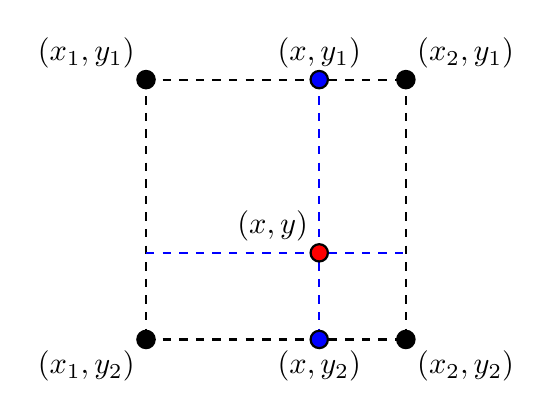
\begin{tikzpicture}[thick,scale=1.1, every node/.style={transform shape}]
        \draw[thick,dashed] (-2,2) -- (1,2);
        \draw[thick,dashed] (-2,2) -- (-2,-1);
        \draw[thick,dashed] (1,2) -- (1,-1);
        \draw[thick,dashed] (-2,-1) -- (1,-1);
        \draw[fill] (-2,2) circle (0.1) node[anchor=south east] {$(x_1,y_1)$};
        \draw[fill] (1,2) circle (0.1) node[anchor=south west] {$(x_2,y_1)$};
        \draw[fill] (-2,-1) circle (0.1) node[anchor=north east] {$(x_1,y_2)$};
        \draw[fill] (1,-1) circle (0.1) node[anchor=north west] {$(x_2,y_2)$};
        
        \draw[thick,blue,dashed] (0,2) -- (0,-1);
        \draw[thick,blue,dashed] (-2,0) -- (1,0);
        \draw[fill=red] (0,0) circle (0.1) node[anchor=south east] {$(x,y)$};
        \draw[fill=blue] (0,2) circle (0.1) node[anchor=south] {$(x,y_1)$};
        \draw[fill=blue] (0,-1) circle (0.1) node[anchor=north] {$(x,y_2)$};
    \end{tikzpicture}

    \caption{The point $(x,y)$ and its neighboring points, which are used to approximate $f(x,y)$ by bilinear interpolation}
    \label{fig:bilinear}
\end{figure}

\paragraph{Approximately the same number of points as pixels.}
If the number of points is approximately the same as the number of pixels in the image, then bilinear interpolation can be used for each point.

First, the four pixels of the image that are closest to the given point $(x,y)$ are determined. These four points form a square. Then, the weighted average of these points is calculated along the $x$ axis, giving approximate function values at two points, which only differ in their $y$ coordinate. Finally, the weighted average of the function values at these points is calculated to get the approximation of $f(x,y)$. The points involved in this interpolation are shown on Figure~\ref{fig:bilinear}.



\paragraph{Much less points than the number of pixels.}
If the number of points is far fewer than the number of pixels, then using bilinear interpolation many of the original pixel values would not be represented in the final approximate function values. Therefore, the following algorithm is used to approximate function values using discrete integration.

First, for each pixel in the original image, determine which point it falls closest to after the linear transformation. Then, for each point in the discrete orthogonal points system, calculate the average of the pixels that are closest to that point. This algorithm divides the unit disk into annular sections based on the proximity to the new points. This is shown on Figure~\ref{fig:interpolation_integral}.

\begin{figure}[tb]
    \begin{subfigure}{.45\textwidth}
    \centering
    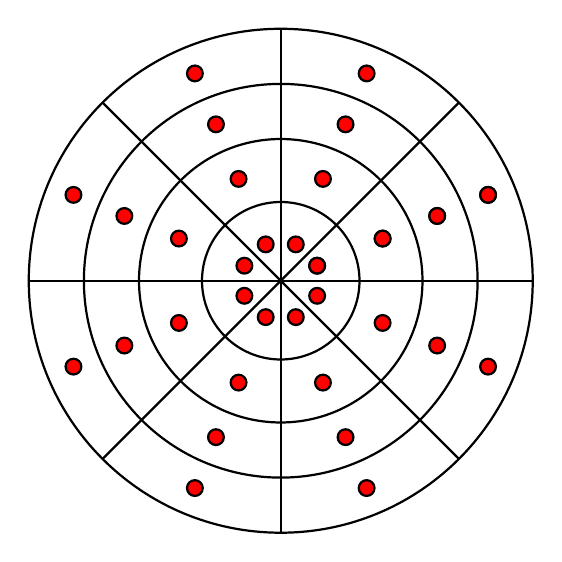
\begin{tikzpicture}[thick,scale=1, every node/.style={transform shape}]
        \foreach \r in {1,1.8,2.5,3.2}
            \draw (0,0) circle (\r);
        \foreach \x in {0,45,...,360} {
            \draw[thick] (0,0) -- (\x:3.2);
            \foreach \r in {0.5,1.4,2.15,2.85}
                \draw[fill=red] (22.5+\x:\r) circle (0.1);
        }
    \end{tikzpicture}

    \caption{The points system on the unit disk and the annular sectors over which the pixel values are averaged.}
    \end{subfigure}
    \hspace{.05\textwidth}
    \begin{subfigure}{.45\textwidth}
        \centering
        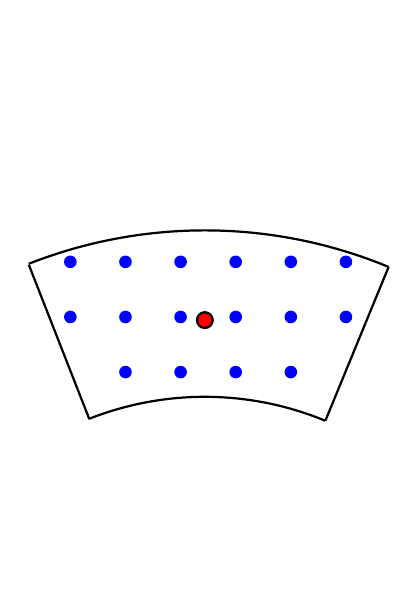
\begin{tikzpicture}[thick,scale=1, every node/.style={transform shape}]
            \draw (6.1*0.3826,6.1*0.9304) arc (67.5:111.5:6.1);
            \draw (4*0.3826,4*0.9304) arc (67.5:111.5:4);
            \draw (4*0.3826,4*0.9304) -- (6.1*0.3826,6.1*0.9304);
            \draw (-4*0.3665,4*0.935) -- (-6.1*0.3665,6.1*0.935);
            \foreach \x in {0,1,...,3} {
                \foreach \y in {2,3,...,4} {
                    \fill[color=blue] (0.7*\x-0.7*1.44,0.7*\y+0.7*4.2) circle (0.08);
                }
            }
            \fill[color=blue] (-0.7-0.7*1.44,0.7*3+0.7*4.2) circle (0.08);
            \fill[color=blue] (-0.7-0.7*1.44,0.7*4+0.7*4.2) circle (0.08);
            \fill[color=blue] (4*0.7-0.7*1.44,0.7*3+0.7*4.2) circle (0.08);
            \fill[color=blue] (4*0.7-0.7*1.44,0.7*4+0.7*4.2) circle (0.08);
            \draw[fill=red] (90:5) circle (0.1);
            \draw[color=white] (0,2) circle (0.1);
            \draw[color=white] (0,8.60) circle (0.1);
        \end{tikzpicture}
    
        \caption{A single annular sector with the original image pixels (blue) and the point in which the approximate function value has to be calculated (red).}
        \end{subfigure}
        \caption{}
    \label{fig:interpolation_integral}
\end{figure}

The comparison between one of the original transformations and the two methods for approximating function values is shown on Figure~\ref{fig:pepper_trans} on the peppers image from the USC-SIPI Image Database~\cite{usc_sipi}.

\begin{figure}
    \begin{subfigure}{.49\textwidth}
        \centering
    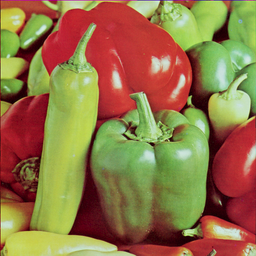
\includegraphics[width=\textwidth]{figures/pepper_color_256.png}
    \caption{Original image}
    \end{subfigure}
    \begin{subfigure}{.49\textwidth}
        \centering
    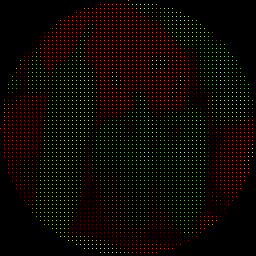
\includegraphics[width=\textwidth]{figures/pepper_square.png}
    \caption{Original transformation}
    \end{subfigure}
    \begin{subfigure}{.49\textwidth}
        \centering
    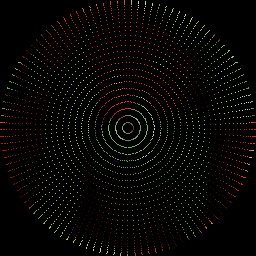
\includegraphics[width=\textwidth]{figures/pepper_bilinear.png}
    \caption{Bilinear interpolation}
    \end{subfigure}
    \begin{subfigure}{.49\textwidth}
        \centering
    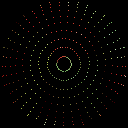
\includegraphics[width=\textwidth]{figures/pepper_integral.png}
    \caption{Interpolation by integrals}
    \end{subfigure}
    \caption{Different transformations with different interpolation methods of the peppers image.}
    \label{fig:pepper_trans}
\end{figure}

\chapter{Tests and comparison with the previous method}
In this chapter we present the different tests that were performed to compare the capabilities of the old and new methods.

In total, four kinds of tests were conducted:
\begin{itemize}
	\item Invariance
	\item Image reconstruction
	\item Image recognition
	\item Template matching
\end{itemize}
All of these tests were run for both the old and new methods and the results have been compared.

\section{Invariance}

\section{Image reconstruction}

\section{Image recognition}

\section{Template matching}


\chapter{Conclusion}
\label{sec:conclusion}
In this chapter we summarize the work and results presented in this thesis. We also present a short overview of further possibilities based on this work.

We have constructed a points system on the unit disk, over which the quaternion extension of the Zernike functions is discrete orthogonal. Using this method of discretization, the quaternion Zernike moments are more robust to noise than with the previously used method.

Many tests have been performed on large sets of images to verify and quantify the improvements of the method.
First, the invariance properties of the QZMIs have been verified empirically using the proposed method.

By comparing the image reconstruction capabilities of the original and the proposed method, we found that the mean square error of reconstruction can decrease significantly, by more than 50\% in some cases, when using the proposed method.

Significant improvements in image recognition have also been achieved by the new method, especially under highly noisy environments. With respect to Gaussian noise the new method is much more robust, achieving a recognition rate of more than 80\% even for extreme noise values, where the original method only achieved a rate of recognition of around 15\%. The reason for this improvement is that due to the discrete orthogonality property of the new method, there is no redundancy between different moments.

With respect to salt-and-pepper noise, no significant difference could be determined between the methods, since this kind of noise adds a very high frequency component to the image, which is filtered by using only moments with low orders in both methods.

We have also found that in order to achieve almost the same recognition rate with the new method as the original one, the number of points in the system can be reduced to almost the minimum number required to still achieve discrete orthogonality. This reduces the computational costs significantly. 

\section{Future possibilities}
One possibility for future work is to employ the techniques described in this thesis in some applications, which currently use other Zernike moment based methods.

It is also possible to utilize the techniques described in this thesis to try and improve other quaternion moment invariant based methods, such as the quaternion Fourier-Mellin moments~\cite{qfmm}.

Finally, the methods described could be further generalized to three dimensional space, where possible applications include pattern recognition in point clouds produced by LiDAR sensors~\cite{zernike_lidar}.

\chapter*{Acknowledgment}
The project was made possible by the support of the European Union and the cofunding of the European Social Fund (EFOP-3.6.3-VEKOP-16-2017-00001)
\usetikzlibrary{backgrounds,calc}
\begin{tikzpicture}[remember picture,overlay]
  \begin{pgfonlayer}{background}
    \node[anchor=south east,outer sep=0pt,inner sep=0pt] at (current page.south east) {
\includegraphics[width=12cm]{figures/efop_logo.png}};
  \end{pgfonlayer}
\end{tikzpicture}

% A projekt az Európai Unió támogatásával, az Európai Szociális Alap társfinanszírozásával valósult meg (EFOP-3.6.3-VEKOP-16-2017-00001).


%%%%%%%%%%%%%%%%%%%%%%%%%%%%%%
%% Bibliography starts here %%

\addcontentsline{toc}{chapter}{Bibliography}

%% There's more than one way to keep track of your citations.

%% For simply listing the citations by text you can use the thebibliography 
%% environment. See biblio.tex for an example. Comment out the following line
%% to use this style.
  
% \input{biblio.tex}


%% Another way is to use bibtex. The following command will process and 
%% include the citations listed in biblio.bib. The advantage of bibtex is that
%% you can simply copy-paste citations if the authors provided a bib-citation. 
%% For examples of such bib-citations, click the small "bib" link beside the 
%% articles at  https://plc.inf.elte.hu/erlang/refactorerl-academic-results.html

\bibliography{biblio}{}
\bibliographystyle{unsrtnat}

%%%%%%%%%%%%%%%%%%%%%%%%%%%%
%% Appendices starts here %%

%\addtocontents{toc}{\setcounter{tocdepth}{0}}
%\input{appendix.tex}
\end{document}
